\documentclass{article}
\usepackage{preamble}
\usepackage{geometry}

 \geometry{
 a4paper,
 total={170mm,257mm},
 left=20mm,
 top=20mm,
 }
 \usepackage{graphicx}
 \usepackage{titling}

 \title{Манипуляции с Pandas для анализа данных}
 \author{Пицик Харитон 211гр.}
\date{}
 
 \usepackage{fancyhdr}
\makeatletter
\def\@maketitle{%
  \newpage
  \null
  \vskip 1em%
  \begin{center}%
  \let \footnote \thanks
    {\LARGE \@title \par}%
    \vskip 1em%
    %{\large \@date}%
  \end{center}%
  \par
  \vskip 1em}
\makeatother

\usepackage{lipsum}  
\usepackage{cmbright}

\begin{document}

\maketitle

\noindent\begin{tabular}{@{}ll}
    Авторство & \theauthor\\
\end{tabular}

\section*{Введение: что такое Pandas \& почему Pandas?} 
Pandas "--- библиотека, являющаяся надстройкой над NumPy и предназначенная для обработки табличных данных и временных рядов. (Интересный факт: название библиотеки происходит от слова <<панельные данные>>. Панельные данные - это многомерные данные, полученные в результате серий наблюдений для одних и тех же людей / компаний (термин из эконометрики)). 

Pandas обеспечивает работу с данными в рамках среды Python, что позволяет не переключаться на изначально более специализированные инструменты, такие как R.

\section*{FunFact: как Pandas отрисовывает таблицы?}
В Pandas отрисовка красивых таблиц (обычно это то, что вы видите) в интерактивных средах, таких как Jupyter Notebook (дальнейшее описание подразумевает, что мы работаем именно в нём), реализована с помощью HTML"=рендеринга. В Pandas за это отвечает система repr"=методов и форматтеров. Как это работает: у объекта DataFrame (например) при вызове функции вывода (head, tail, etc.) срабатывает внутренний метод \_repr\_html\_(). Этот метод возвращает HTML"=таблицу с заголовками, ну в общем вы понимаете о чём я. repr довольно уникальная штука, вот поддерживаемые методы:
\begin{enumerate}
    \item \_\_repr\_\_() "--- то, что выводится в консоль;
    \item \_repr\_html\_() "--- HTML представление;
    \item \_repr\_latex\_() "--- \LaTeX представление (!!! если поддерживается !!!);
    \item и т.д.
\end{enumerate}

В модуле pandas.io.formatter определены методы для декорирования таблиц. В рамках этой лекции я лишь упомяну \textbf{styles.Styler}, который предоставляет возможность кастомизировать визуал с помощью CSS шаблонов. Упомнял я его чтобы уточнить: даже без Styler, вывод DataFrame даёт <<приятный>> визуал, т.к. при выводе в любом случае вызывается вышеупомянутый \_repr\_html\_().


\section*{Считываем данные}
Считывание .csv (comma separated values) таблицы "--- pd.read\_csv(). На этом можно было бы закончить лекцию, но данные бывают большими: под большими я подразумеваю просто гигантские, которые по размеру будут серьёзными для нашего компьютера. В pandas мы можем загружать данные чанками (возможно, у кого"=то в голове сейчас откликнутся итераторы из Python). 

В общем суть такая: нам нужно считывать данные чанками. Сделать это можно с помощью ключевого слова \textit{chunksize} для команды \textit{pd.read\_csv()}.

\begin{minted}[style=bw]{python}
for chunk in pd.read_csv('data.csv', chunksize=10000):
    chunk.to_csv('chunked_file.csv', mode = 'a', index = False, header = False)
\end{minted}

Обратим также внимание на сам объект (как вы могли догадаться, он итерируемый):
\begin{minted}[style=bw]{python}
chunk = pd.read_csv('data.csv', chunksize = 10000)
type(chunk) #pandas.io.parsers.readers.TextFileReader
\end{minted}

readers.TextFileReader получается в результате read\_csv или read\_table и позволяет читать огромные CSV-файлы по частям, не загружая всё сразу в память. chunk "--- \textit{итерируемый}, т.е. мы можем запихнуть это в цикл for, а можем получать по одному с помощью метода get\_chunk().

\begin{minted}[style=bw]{python}
#read_table vs read_csv
#помогает для считывание tsv (tab-separated values)
pd.read_table("file.txt")  =  pd.read_csv("file.txt", sep="\t")
\end{minted}

\section*{Оптимизация типов данных}
Pandas по умолчанию загружает данные с типами, которые не всегда эффективны. Например, столбцы с числами могут загружаться как float64, даже если достаточно float32, а категориальные данные хранятся как object, вместо category.

Проверить текущие типы данных можно с метода df.dtypes.
Самый очевидный (и удобный) способ приведения типов "--- функции Pandas:
\begin{minted}[style=bw]{python}
df['col'] = df['col'].astype(int)

df[['col1', 'col2']].astype(int)

df.astype({'col1': int, 'col2': int, 'col3': float})

#еще есть метод to_numeric (unsigned int)
df['col'] = pd.to_numeric(df['col'], errors = 'coerce')

#Если в столбце много повторяющихся значений, category может сэкономить память
df['category_column'] = df['category_column'].astype('category')

#Если явно не указано явно, Pandas преобразует даты в object.
df['date'] = pd.to_datetime(df['date'], errors='coerce')


#Если много разреженных типов, можем смело использовать SparseArray
df['sparse_column'] = pd.arrays.SparseArray(df['dense_column'])
\end{minted}

Также для оптимизации типов поддерживается pyarrow:
\begin{minted}[style=bw]{python}
df['col'] = df['col'].astype('string[pyarrow]')
\end{minted}
так Pandas использует тип Arrow-backed string dtype, которые эффективные (за счёт поддержки ранее обсуждаемой SIMD) и хранятся в бинарном формате.

Есть метод convert\_dtypes, который пытается сам преобразовать типы в наиболее подходящие согласно иерархии типов.

\section*{Векторизация для операций Pandas (numba, cython)}
Раз уж мы начали обсуждать что"=то, связанное с оптимизацией, давайте рассмотрим, как применется векторизация в Pandas. (Вернее, ускорение операций)

\subsection*{Numba}
Numba ускоряет непосредственно сам Python. Он является JIT"=компилятором (just"=in"=time, динамическая компиляция "--- технология, в которой байт"=код преобразовывается в машинный непосредственно во время работы программы), который <<очень любит>> циклы и работу с NumPy. Давайте рассмотрим примитивный кейс использования numba. Перед этим добавлю, что Numba переводит подмножество NumPy и Python операций в машинный код оптимизированным способом через LLVM (low level virtual machine) с помощью пакета llvmlite для Python.
\begin{minted}[style=bw]{python}
import pandas as pd
import numba
#100.000 строк, 4 колонки
df = pd.DataFrame(np.random.randint(0,100,size=(100000, 4)),columns=['a', 'b', 'c', 'd'])

def add_new_col(x):
    return x * 5

@numba.vectorize
def add_new_col_numba(x):
    return x * 5
\end{minted}

Результаты следующие:
\begin{minted}[style=bw]{python}
# наша функция
In [1]: %timeit df['new_col'] = df['a'].apply(multiply)
23.9 ms ± 1.93 ms per loop (mean ± std. dev. of 7 runs, 10 loops each)

# встроенная имплементация Pandas
In [2]: %timeit df['new_col'] = df['a'] * 5
545 µs ± 21.4 µs per loop (mean ± std. dev. of 7 runs, 1000 loops each)

# наша функция с numba
# мы отдаем весь вектор значений, чтобы numba сам провел оптимизацию цикла
In [3]: %timeit df['new_col'] = multiply_numba(df['a'].to_numpy())
329 µs ± 2.37 µs per loop (mean ± std. dev. of 7 runs, 1000 loops each)
\end{minted}

Таким образом, <<оптимизированная>> версия быстрее в ~70 раз! Однако в случаее абсолютных величин, реализация в Pandas не сильно отстала от numb'ы. Давайте рассмотрим более сложный кейс:
\begin{minted}[style=bw]{python}
# возводим значения строки в квадрат и берем их среднее 
def square_mean(row):
    row = np.power(row, 2)
    return np.mean(row)
# применение:
# df['new_col'] = df.apply(square_mean, axis=1)

# numba не умеет работать с примитивами pandas (Dataframe, Series и тд.)
# поэтому мы даем ей двумерный массив numpy
@numba.njit
def square_mean_numba(arr):
    res = np.empty(arr.shape[0])
    arr = np.power(arr, 2)
    for i in range(arr.shape[0]):
        res[i] = np.mean(arr[i])
    return res
# применение:
# df['new_col'] = square_mean_numba(df.to_numpy())
\end{minted}

По этому графику мы видим, что результаты уже разительно отличаются:
\begin{figure}[H]
    \centering
    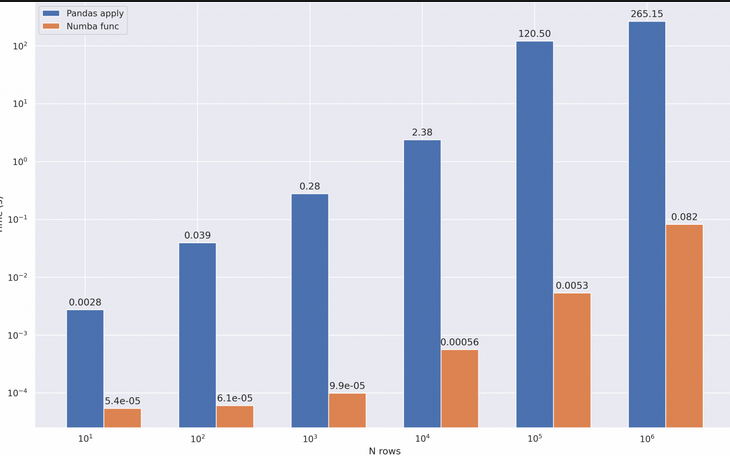
\includegraphics[width=0.75\linewidth]{pandas_numba.png}
    \caption{Numba vs. Pandas}
\end{figure}

\subsection*{Cython}
В большинстве случаев, конечно, Python и NumPy хватает для большинства вычислительных процессов, однако если они становятся слишком вычислительно сложными или просто требуется их ускорить, применяется модуль \textbf{Cython}.


Рассмотрим следующий блок кода, в котором мы реализуем функцию для дальнейшего \textbf{.apply}:
\begin{minted}[style=bw]{python}
In [3]: def f(x):
   ...:     return x * (x - 1)
   ...: 

In [4]: def integrate_f(a, b, N):
   ...:     s = 0
   ...:     dx = (b - a) / N
   ...:     for i in range(N):
   ...:         s += f(a + i * dx)
   ...:     return s * dx
   ...: 
\end{minted}

Получим следующее время:
\begin{minted}[style=bw]{python}
In [5]: %timeit df.apply(lambda x: integrate_f(x["a"], x["b"], x["N"]), axis=1)
84 ms +- 1.01 ms per loop (mean +- std. dev. of 7 runs, 10 loops each)
\end{minted}
С помощью функции IPython \textbf{prun} можно убедиться, что большая часть времени теряется именно в этих функциях.

Теперь давайте скопируем нашу функцию, но под Cython:
\begin{minted}[style=bw]{python}
In [8]: %%cython
   ...: def f_plain(x):
   ...:     return x * (x - 1)
   ...: def integrate_f_plain(a, b, N):
   ...:     s = 0
   ...:     dx = (b - a) / N
   ...:     for i in range(N):
   ...:         s += f_plain(a + i * dx)
   ...:     return s * dx
   ...: 
\end{minted}

Результат:
\begin{minted}[style=bw]{python}
In [9]: %timeit df.apply(lambda x: integrate_f_plain(x["a"], x["b"], x["N"]), axis=1)
47.2 ms +- 366 us per loop (mean +- std. dev. of 7 runs, 10 loops each)
\end{minted}

\section*{Индексация и отличия от NumPy}
Pandas предоставляет несколько вариантов индексации, почему бы нам об этом не поговорить.

\subsection*{LOC, ILOC}
Индексация по локальному и фактическому индексам, позволяет выбрать набор строк / столбцов по заданным \textit{лейблам}.

ILOC позволяет индексировать, по факту, как мы привыкли индексировать массивы (начиная с 0 и т.д.). Это ещё называется \textit{неявной индексацией}. Давайте быстренько рассмотрим пример:
\begin{minted}[style=bw]{python}
>>> mydict = [{'a': 1, 'b': 2, 'c': 3, 'd': 4},
...           {'a': 100, 'b': 200, 'c': 300, 'd': 400},
...           {'a': 1000, 'b': 2000, 'c': 3000, 'd': 4000}]
>>> df = pd.DataFrame(mydict)
>>> df
      a     b     c     d
0     1     2     3     4
1   100   200   300   400
2  1000  2000  3000  4000


>>> df.iloc[[0]]
   a  b  c  d
0  1  2  3  4
>>> type(df.iloc[[0]])
<class 'pandas.core.frame.DataFrame'>
\end{minted}

LOC же, в свою очередь, является \textit{явной индексацией}. Грубо говоря это означает, что мы можем использовать индексы, которые видим в таблице. Опять же, рассмотрим пример
\begin{minted}[style=bw]{python}
>>> df = pd.DataFrame([[1, 2], [4, 5], [7, 8]],
...                   index=['cobra', 'viper', 'sidewinder'],
...                   columns=['max_speed', 'shield'])
>>> df
            max_speed  shield
cobra               1       2
viper               4       5
sidewinder          7       8

>>> df.loc['viper']
max_speed    4
shield       5
Name: viper, dtype: int64
\end{minted}

FunFact: в более ранних версиях Pandas есть метод .x, который позволяет объединять .loc и .iloc в одну индексацию.

\subsection*{AT, IAT}
Метод at позволяет получить \textbf{один} элемент, находящийся на пересечении выбранных строки и столбца и делает это \textit{явно}, по аналогии с loc:
\begin{minted}[style=bw]{python}
df = pd.DataFrame([[0, 2, 3], [0, 4, 1], [10, 20, 30]],
                  index=[4, 5, 6], columns=['A', 'B', 'C'])
df
>>  A   B   C
4   0   2   3
5   0   4   1
6  10  20  30

df.at[4, 'B']
>> 2

#тоже самое
df.loc[4].at['B']
>> 2
\end{minted}

iat, как вы могли догадаться, позволяет делать то же самое но по \textit{неявному} индексу:
\begin{minted}[style=bw]{python}
df = pd.DataFrame([[0, 2, 3], [0, 4, 1], [10, 20, 30]],
                  columns=['A', 'B', 'C'])

df
>>  A   B   C
0   0   2   3
1   0   4   1
2  10  20  30

df.iat[1, 2]
>> 1
\end{minted}
+
 
\subsection*{MultiIndex}
Объект MultiIndex позволяет воспроизвести более сложные конструкции, например:
\begin{minted}[style=bw]{python}
index = [('California', 2000), ('California', 2010),
         ('New York', 2000), ('New York', 2010),
         ('Texas', 2000), ('Texas', 2010)]
         
populations = [33871648, 37253956,
               18976457, 19378102,
               20851820, 25145561]

               
data = pd.Series(populations, index=index)
index = pd.MultiIndex.from_tuples(index)
data = data.reindex(index)
data

>> California  2000    33871648
               2010    37253956
   New York    2000    18976457
               2010    19378102
   Texas       2000    20851820
               2010    25145561
   dtype: int64
\end{minted}

Можно думать, что MultiIndex "--- это некое новое измерение наших данных. Вы могли бы заметить, что вообще"=то, мы могли бы представить наши данные и без подобного <<оверхеда>>, но иногда представление мультииндексом бывает полезным:
\begin{minted}[style=bw]{python}
data_df = data.unstack()
data_df
\end{minted}

\begin{figure}
    \centering
    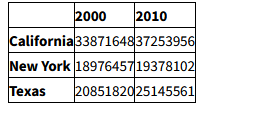
\includegraphics[width=0.55\linewidth]{unstack.png}
    \caption{unstack (прошу прощения за качество)}
    \label{fig:enter-label}
\end{figure}

\section*{Обработка NaN значений}
\subsection*{Как в целом это устроено}
Зачастую приходиться обрабатывать так называемые Na значения в данных, но что вы вообще понимаете под 
Na? Одинаковые ли они все? Как Pandas отличает Na от реально существующих данных?

Давайте рассмотрим 2 схемы, по которым ЯП определяют отсутствие данных: использование маски, которая глобально идентифицирует отсутствующие данные, или какое"=то заданное значение для каждого типа (\textit{сигнальный} метод).

В случае маскирования, сама маска представляет собой булевый массив, или же может присваивать бит в представлении данных там, <<где их нет>> (для локального указания нулевого статуса значения).

В сигнальном методе, как я уже и говорил, применяется специальное значение для обозначения отсутствующей даты (например, -9999 для int или любой другой, более сложный паттерн). Например, это также может быть NaN для типов с плавающей точкой, по соглашению института инженеров электротехники и электроники (IEEE).

Возможно вы догадываетесь, но здесь нет во всём хорошего решения. В случае с масками, необходимо аллоцировать память под дополнительный булевый массив, размерность которого совпадает с датасетом, что понятное дело добавляет оверхеда для итак непростой задачи. Сигналы же ограничивают область значений типа, что может вовлечь за собой дополнительную (часто неоптимизированную) логику вычислений в CPU (и GPU). Возвращаясь к первому предложению (нет хорошего во всём решения), дополню, что разные языки используют разные соглашения. Не ходя далеко от темы, язык R использует зарезервированные битовые шаблоны в каждом типе данных как сигнальные значения, указывающие на отсутствие данных.

\subsection*{Наконец"=то возвращаемся к пандам}
Способ, которым Pandas обрабатывает отсутствующие значения, ограничен его зависимостью от пакета NumPy, который не имеет встроенного понятия значений NA для типов данных, не являющихся точками с плавающей запятой. Pandas решил использовать sentinels для недостающих данных и далее решил использовать два уже существующих в Python нулевых значения: специальное значение NaN с плавающей точкой и объект Python None. 

Всё что пока"=что нам нужно знать про None из Python, что это если вы решите аггрегировать / проитерироваться на объекте с None внутри "--- вы вылетите в ошибку. np.nan же в свою очередь работает как вирус: любой метод, возвращающий что"=либо (кроме специализированных) и хоть как"=то взаимодействующий с np.nan вернёт np.nan:
\begin{minted}[style=bw]{python}
arr = np.array([np.nan, 2, 3, 4])
arr.min(), arr.max(), arr.sum()
\end{minted}
Встречаем специализированные методы:
\begin{minted}[style=bw]{python}
arr = np.array([np.nan, 2, 3, 4])
arr.nanmin(), arr.nanmax(), arr.nansum()
\end{minted}
Обратите внимание на следующий каст в Python:
\begin{minted}[style=bw]{python}
x = pd.Series(range(2), dtype=int)
x
>>0    0
  1    1
  dtype: int64

x[0] = None
x
>> 0    NaN
   1    1.0
   dtype: float64
\end{minted}

\subsection*{Команды для обработки пропущенных значений }
\begin{minted}[style=bw]{python}
data = pd.Series([1, np.nan, 'hello', None])
data.isnull()
>> 0    False
   1     True
   2    False
   3     True
   dtype: bool

data[data.notnull()]
>>  0        1
    2    hello
    dtype: object
    
data.dropna()
>> 0        1
   2    hello
   dtype: object
\end{minted}
Здесь затронуты примитивные команды, но на dropna и fillna (см. ниже) хочу остановиться подробнее.

Для dropna хочу акцентировать внимание на ключевых словах \textbf{thresh} и \textbf{how}. Thresh "--- принимает int и означает минимальное количество непустых значений, при котором строка / столбец \textit{не удаляется}. How (по умолчанию 'any') означает <<стратегию>>, по которой будут удаляться строки / столбцы. При значении 'all' удалятся только те строки / столбцы, которые везде содержат пустоту.
\begin{figure}[H]
    \centering
    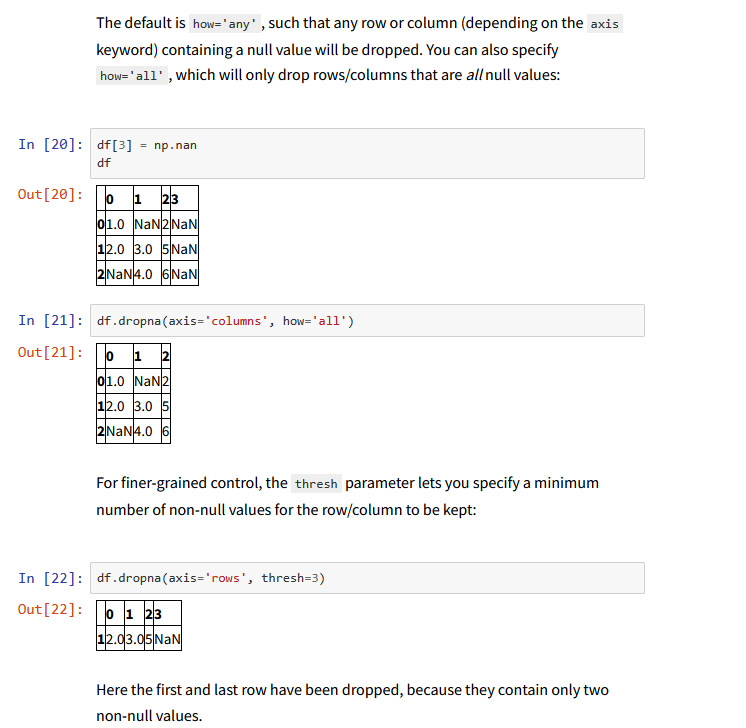
\includegraphics[width=0.85\linewidth]{изображение.png}
    \caption{dropna}
    \label{fig:enter-label}
\end{figure}

Также есть метод fillna который просто заполняет пустые значения указанным значением. Однако стоит уточнить про его ключевое слово method, которое позволяет выбрать стратегию как именно заполнять. например, method='ffil' (forward"=fill) позволяет <<толкать вперёд>> предыдущее значение (угадайте что делает bfill) (Для этих методов можно указывать ось, для fillna с method это особенно имеет смысл писать явно).

\section*{Слияние и конкатенация}
Давайте рассмотрим методы и стратегии конкатенации, слияния данных.
\subsection*{Concat}
pd.concat, как можно было догадаться, просто конкатенирует данные относительно заданной оси 
\begin{minted}[style=bw]{python}
ser1 = pd.Series(['A', 'B', 'C'], index=[1, 2, 3])
ser2 = pd.Series(['D', 'E', 'F'], index=[4, 5, 6])
pd.concat([ser1, ser2])

>>  1    A
    2    B
    3    C
    4    D
    5    E
    6    F
    dtype: object
\end{minted}
Удивительно, но факт: это также работает с DataFrame. Однако здесь стоит обратить внимание:
индексация не сохраняется, и её приходится перезаписывать... могли бы подумать вы, однако можно (если это будет удобно) прописать ключевое слово ignore\_index:
\begin{minted}[style=bw]{python}
pd.concat([df_x, df_y], ignore_index = True)
\end{minted}

\begin{figure}[H]
    \centering
    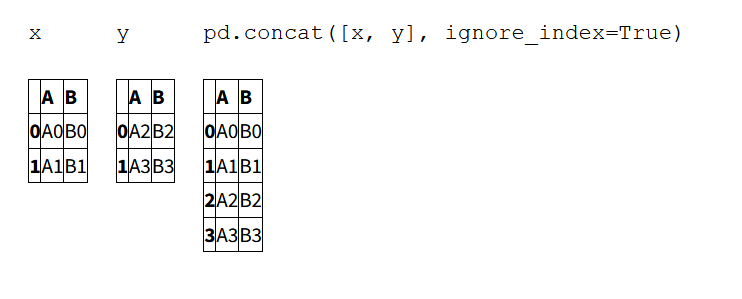
\includegraphics[width=0.65\linewidth]{concat_index.png}
    \caption{Конкатенация без конфликтов по индексу}
    \label{fig:enter-label}
\end{figure}

Можно указать метод join, который позволяет указать метод присоединения, например \mintinline{python}{join='inner'} означает, что будут объединены только пересекающиеся колонки. Также просто упомяну метод \mintinline{python}{join_axes}, в котором можно указать, по каким строкам / столбцам будет оформлено присоединение.


\subsection*{Merge}
Для объединения данных есть ещё продвинутые методы, один из таких "--- merge. С ним немного посложнее, так как в зависимости от ситуации нужно понимать, как именно он соединит данные. Рассмотрим основные ситуации (надеюсь никто ещё не расстраивается, что я беру готовые мини"=датасеты):
\subsubsection*{Один"=к"=одному}
\begin{figure}[H]
    \centering
    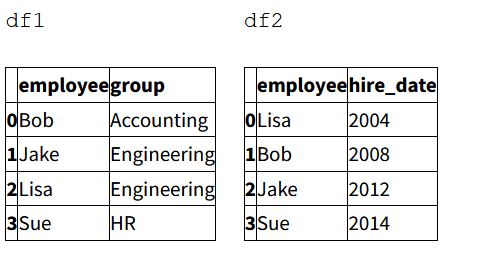
\includegraphics[width=0.45\linewidth]{merge_onebyone.png}
    \caption{Один к одному}
    \label{fig:enter-label}
\end{figure}
\begin{figure}[H]
    \centering
    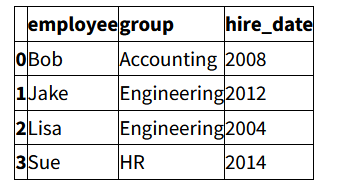
\includegraphics[width=0.45\linewidth]{merge_onebyone_result.png}
    \caption{Результат}
    \label{fig:enter-label}
\end{figure}
В целом это самый простой случай объединения. Всё можно понять по картинкам.

\subsubsection*{Многие"=к"=одному}
\begin{figure}[H]
    \centering
    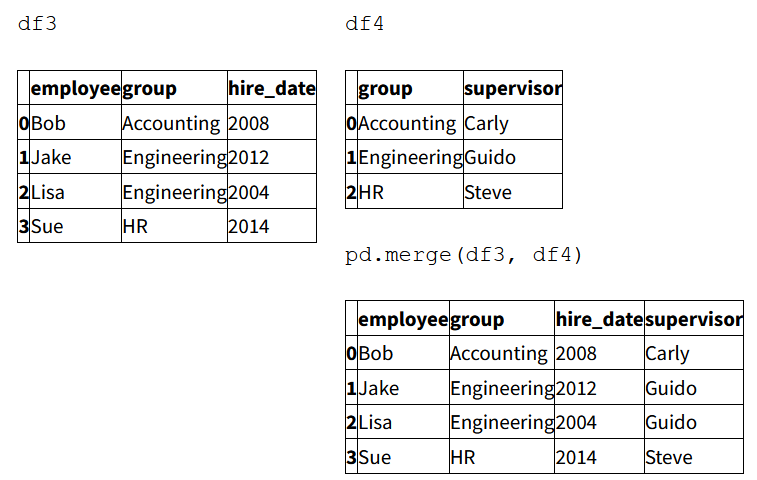
\includegraphics[width=0.6\linewidth]{merge_manybyone.png}
    \caption{Многие к одному}
    \label{fig:enter-label}
\end{figure}
Многие к одному "--- случай, когда один из датасетов содержит дубликаты в столбце"=ключе (общий столбец, по которому объединяются данные. В тривиальных случаях Pandas определяет их самостоятельно, но всё равно лучше прописывать явно с помощью ключевого слова on). В этом случае возвращается DataFrame с сохранёнными дубликатами.
\subsubsection*{Многие"=к"=многим}
Ситуация, когда обе ключевые колонки объединяемых датасетов содержат дубликаты:
\begin{figure}[H]
    \centering
    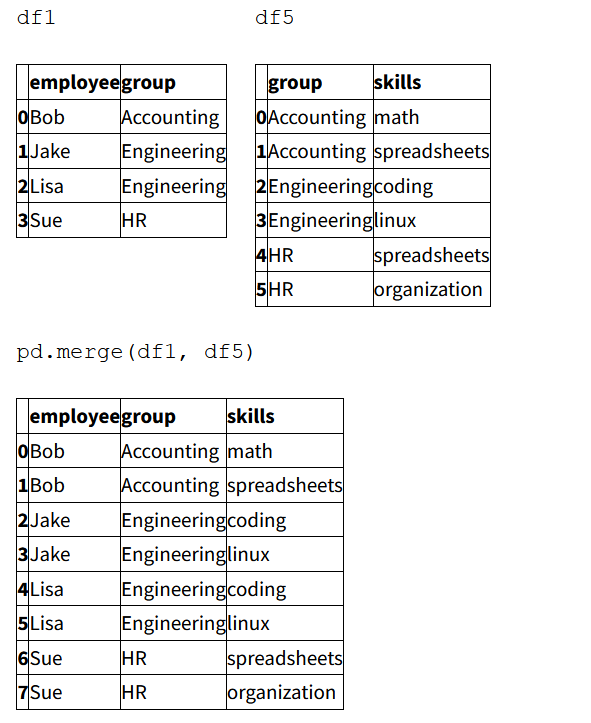
\includegraphics[width=0.52\linewidth]{merge_manytomany.png}
    \caption{Многие к многим}
    \label{fig:enter-label}
\end{figure}

В качестве некой <<модификации>> ключевого слова on есть методы \mintinline{python}{left_on, right_on}. Они пригождаются, когда ключевые колонки в разных датасетах имеют разные названия. Тогда мы указываем для left\_on колонку из датасета, \textbf{к которому} хотим слить данные, а для right\_on колонку из датасета, \textbf{который} хотим слить с исходным.
\section*{Продвинутая трансформация данных}
\subsection*{Объект GroupBy и метод groupby}
Тут не такая простая тема, как может показаться на первый взгляд.

Иногда (часто) нам удобно аггрегировать по заданному индексу / лейблу. С этой задачей нам может помочь метод groupby. Подкованные люди могли заметить, что это рефернс на SQL, где также есть groupby (и join и merge, в этом плане в целом они похожи). Как происходит groupby:
\begin{enumerate}
    \item разделение по значению выбранного ключа / индекса;
    \item применение аггрегирующей функции;
    \item слияние разделившихся данных в результат.
\end{enumerate}
Давайте рассмотрим подробнее. В этом нам поможет следующая картинка:
\begin{figure}[H]
    \centering
    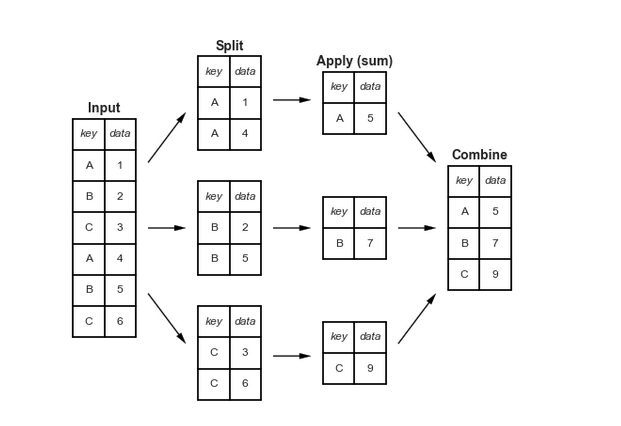
\includegraphics[width=0.75\linewidth]{groupby_structure.png}
    \caption{GroupBy}
    \label{fig:enter-label}
\end{figure}

Важно уточнить, что сам по себе groupby не вернёт ничего, а если быть точнее, то вернётся...
\begin{minted}[style=bw]{python}
<pandas.core.groupby.DataFrameGroupBy object at 0x117272160>
\end{minted}
...DataFrameGroupBy object. Можно думать, что это некоторое подвешенное состояние процедуры, ожидающее применения какой"=то аггрегирующей функции. Если мы решим проиндексировать этот объект, то получим SeriesGroupBy object, суть которого такая же, но разве что возвратом будет Series, а не DataFrame.
\begin{minted}[style=bw]{python}
df = pd.DataFrame({'key': ['A', 'B', 'C', 'A', 'B', 'C'],
                   'data': range(6)}, columns=['key', 'data'])
df.groupby('key').sum()
\end{minted}
\begin{figure}[H]
    \centering
    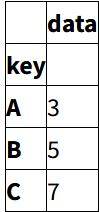
\includegraphics[width=0.15\linewidth]{groupby_return.png}
    \caption{Результат функции}
    \label{fig:enter-label}
\end{figure}

Также на groupby можно проитерироваться, выглядит это как"=то так:
\begin{figure}[H]
    \centering
    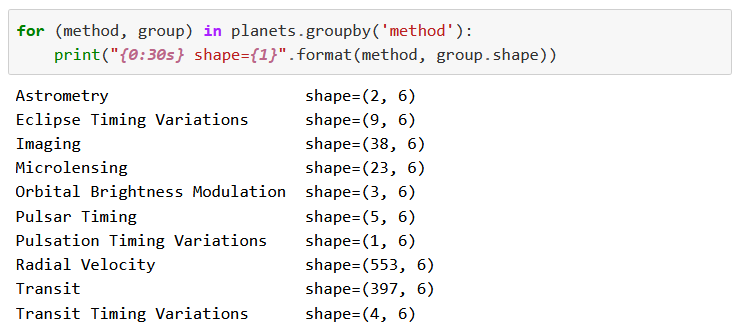
\includegraphics[width=0.7\linewidth]{groupby_iteration.png}
    \caption{Итерация на groupby}
    \label{fig:enter-label}
\end{figure}

\subsection*{Аггрегирование через filter, apply, transform}
\textbf{Apply} метод позволяет применить функцию к столбцу (или создать новый столбец на основе уже существующего). Функция может быть как и предопределённая (min, max...), а может быть <<кастомной>>, которую вы предварительно определили:
\begin{minted}[style = bw]{python}
def plus_five(x):
    return x + 5

df['new_col'] = df['exist_col'].apply(plus_five)
\end{minted}
Это означает, что функция применяется к каждому элементу строки/столбца (в зависимости от аргумента axis), результат функции зависит от определяемой функции (или с помощью ключевого слова result\_type).

\subsection*{Filter}
filter позволяет <<дропнуть>> дату опираясь на заданные признаки. Например, давайте профильтруем данные так, чтобы остались строки, в которых есть стандартное отклонение превышающее 4:
\begin{figure}[H]
    \centering
    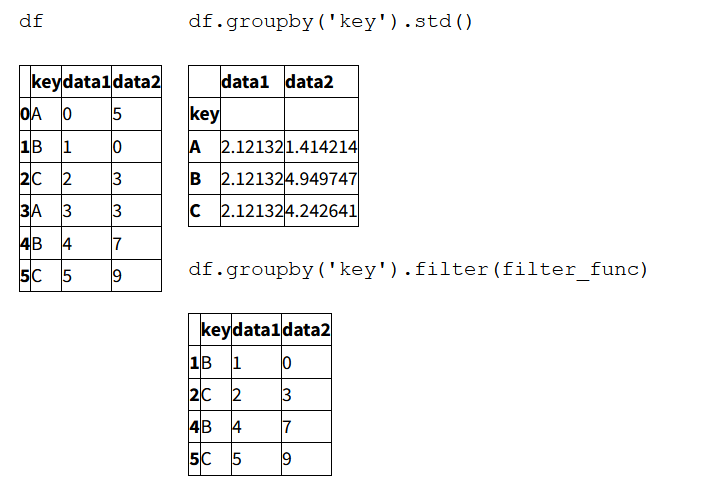
\includegraphics[width=0.75\linewidth]{filter.png}
    \caption{Filter}
    \label{fig:enter-label}
\end{figure}
где filter\_func "--- следующая функция:
\begin{minted}[style=bw]{python}
def filter_func(x):
    return x['data2'].std() > 4
\end{minted}

Метод filter возращает булевый массив и применяет маскирование к исходному датасету, что позволяет вывести только подходящие элементы.

\subsection*{Transform}
До этих пор мы возвращали некоторую уменьшенную, <<отредактированную>> версию данных, однако метод transform позволяет модернизировать исходные. Давайте рассмотрим трансформацию, при которой мы из каждого элемента вычитаем среднее по всему датасету:
\begin{figure}[H]
    \centering
    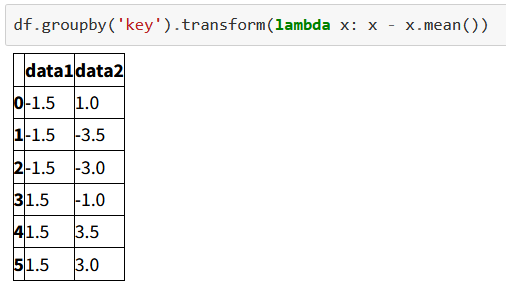
\includegraphics[width=0.75\linewidth]{transform.png}
    \caption{Transform}
    \label{fig:enter-label}
\end{figure}

\section*{Примитивная визуализация}
Инструменты Pandas позволяют применять визуализацию к датасету / продвинутому датасету. Понятное дело, что это лучше делать с помощью специализированных библиотек, таких как Matplotlib.pyplot или Seaborn (или вообще Plotly), но в случае если вам нужен какой"=то график <<на скорую руку>>, можно воспользоваться и Pandas.

Как я уже и говорил, для визуализации существуют более специализированные инструменты, поэтому тут остановимся прям совсем ненадолго. Самое примитивное, что можно сделать "--- метод .plot:

\begin{minted}[style=bw]{python}
np.random.seed(123)

ts = pd.Series(np.random.randn(1000), index = pd.date_range("1/1/2000", periods = 1000))

ts.plot()
\end{minted}

Если же мы применим .plot функцию для DataFrame, то Pandas автоматически раскрасит разные значения в разные цвета. (По факту, .plot функция для Series и DataFrame является некой <<обёрткой>> для аналогичной функции из Matplotlib). Следовательно, существует масса различных графиков, которые можно явно задавать с помощью метода \textbf{kind}. На слайде приведены основные, из названия +- должно быть понятно, какой из них что делает:
\begin{figure}[H]
    \centering
    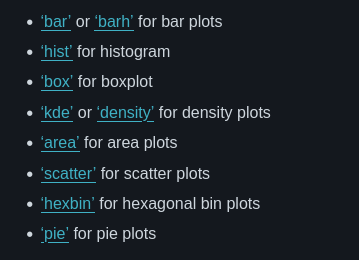
\includegraphics[width=0.75\linewidth]{image.png}
    \caption{plot params}
    \label{fig:enter-label}
\end{figure}

\section*{Заключение}
В принципе на этом всё, что я хотел рассказать про Pandas. Мы успели затронуть что такое в принципе Pandas, как он ускоряет операции и как можно ещё это ускорить, какие основные размышления в нём применются и какую"=никакую примитивную визуализацию.
\end{document}
